\documentclass[cs4size,a4paper,adobefonts,openany]{ctexbook}
\usepackage[colorlinks=true,linkcolor=black]{hyperref}
\usepackage{indentfirst}
\usepackage[a4paper,left=2.5cm,right=2.5cm,bottom=2.5cm,top=2.5cm]{geometry}
\usepackage{fontspec}
\setmainfont{Minion Pro}
\pagestyle{plain}
\punctstyle{kaiming}
%\usepackage{unicode-math}
%\setmathfont{STIX Math}

\usepackage{amsmath,amsthm,amssymb}
\newtheorem{defn}{定义}
\newtheorem{thm}{定理}
\newcommand{\pname}[1]{\underline{#1}}
\numberwithin{equation}{section}
\CTEXsetup[number=\thechapter]{chapter}
\begin{document}
\title{\bfseries Regular Polytopes 的学习笔记}
\author{王盛颐}
\date{}
\maketitle
\setcounter{page}{1}
\chapter{POLYGONS AND POLYHEDRA}
\section{Regular polygons}
假设有 $p$ 个点 $A_1,A_2,\dots,A_p$,那么 $p$ 边形($p$-gon)被定义为连
接这些点的 $p$ 条直线段 $A_1A_2,A_2A_3,\dots,A_pA_1$ 形成的环路。这些线
段和点分别被称为多边形的\pname{边}和\pname{顶点}。目前我们假定所有的边
都不彼此穿插。如果一个多边形所有的顶点都共面,则我们称其为\pname{平面}
多边形,否则称为\pname{斜}多边形。

一个平面多边形将它所在的平面划分为两个区域,面积有限的称为\pname{内部}。
我们通常将这个内部也视作多边形的组成部分,和顶点、边一样。这时平面多边
形可以有另外一个定义,定义为由 $p$ 个不同直线段围成的单连通区域(这里单
  连通区域的意思是区域内任意简单闭曲线都可以连续收缩成一个点)。

有一类平面多边形,特点是任意一条边所在的直线都不穿过多边形内部,这类多
边形特别重要,我们称之为\pname{凸} $p$ 边形,可以用(笛卡尔坐标下)
$p$ 个线性不等式来描述:
\[
a_kx+b_ky \leq c_k\qquad (k=1,2,\dots,p)
\]
这组不等式必须是一致的,没有冗余的,且能据此得到一个有限的积分:
\[
\iint\text{d}x\text{d}y
\]
(这就是多边形的面积)。

一个平面多边形若每条边都相等则被称为等边的,若每个角都相等则被称为等角
的。当 $p>3$ 时,一个平面 $p$ 边形可能等边但不等角,如菱形;也可能等角但
不等边,如长方形。若一个平面 $p$ 边形既等角又等边,则被称之为\pname{正
  则的} (regular),也叫\pname{正} $p$ 边形,记为 $\{p\}$。如 $\{3\}$
是指正三角形,$\{4\}$ 表示正方形,$\{5\}$ 表示正五边形。

很容易看出一个正多边形有一个\pname{中心点},从中心点出发到各个角距离相
等为 ${_0R}$,到各条边距离相等为 ${_1R}$。这意味着两个同心圆,分别是正多边
形的外接圆和内切圆。

有时可以将 $p$ 边形的边认作是首尾相接的 $p$ 个向量。将这些向量的起点并
在一处,则相邻向量的夹角就等于 $p$ 边形的外角,于是 $p$ 边形的外角和为
$2\pi$。那么 $\{p\}$ 的每个外角大小都是 $2\pi/p$,所以每个内角的大小是
\begin{equation}
  (1-\frac{2}{p})\pi
\end{equation}

这也可以从图 \ref{fig:pentagon} 中的直角三角形 $O_2O_1O_0$ 看出来。
$O_2$ 是中心,$O_1$ 是一条边的重点,$O_0$ 是这条边的一个端点。直角在
$O_1$ 处,$O_2$ 处的角度显然是 $\pi/p$。若边长为 $2l$ 则我们有:
\[
O_0O_1=l,\quad O_0O_2={_0R}, \quad O_1O_2={_1R}
\]
因此有
\begin{equation}
  {_0R}=l\csc\frac{\pi}{p}\qquad {_1R}=l\cot\frac{\pi}{p}
\end{equation}

那么 $\{p\}$ 的面积就是这样 $p$ 个三角形的面积和:
\begin{equation}
  C_p = pl\cdot {_1R} = pl^2\cot\frac{\pi}{p}
\end{equation}
周长则是
\begin{equation}
  S=2pl
\end{equation}

\begin{figure}[htbp]
  \centering 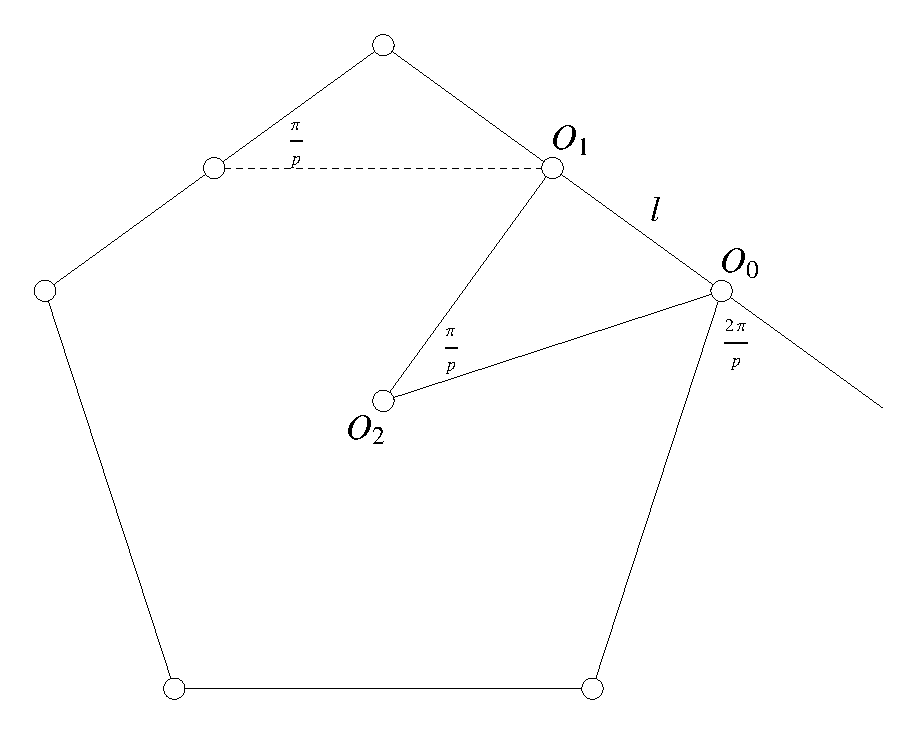
\includegraphics[width=0.7\textwidth]{images/pentagon}
  \caption{正 $p$ 边形的角度长度关系} \label{fig:pentagon}
\end{figure}

当 $p$ 无限增长下去,则 $S/{_0R}$ 和 $S/{_1R}$ 都会渐渐接近 $2\pi$ (阿基米
  德当年就是这么算圆周率的,他计算用的 $p=96$)。

我们也可以计算出 $\{p\}$ 各个顶点的笛卡尔坐标为
\[
\left({_0R}\cos\frac{2k\pi}{p},{_1R}\sin\frac{2k\pi}{p}\right)\qquad(k=0,1,\dots,p-1)
\]

把这些坐标看作复平面上的点,那么外接圆半径 ${_0R}=1$ 的 $\{p\}$ 的顶点可
以认为是分圆方程
\begin{equation}
  z^p=1
\end{equation}
的根 $e^{2k\pi i/p}$。

有时需要扩展 $p$ 边形的定义,允许多边形的边为曲线。比如有时候可能会考虑
\pname{圆多边形},它的边都是球面上大圆的圆弧,这种情况下可以有二边形。

\end{document}
